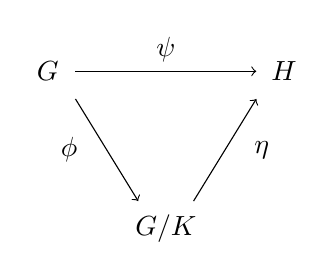
\begin{tikzpicture}[scale=1]

\coordinate (G) at (0,2);
\coordinate (H) at (3,2);
\coordinate (G-mod-K) at (1.5,0);

\coordinate (psi) at (1.5,2);
\coordinate (phi) at (0.5,1);
\coordinate (eta) at (2.5,1);

\node at (G) {$G$};
\node at (H) {$H$};
\node at (G-mod-K) {$G/K$};

\node [above]  at (psi) {$\psi$};
\node [left] at (phi) {$\phi$};
\node [right] at (eta) {$\eta$};

\draw [->] ([xshift=10]G) -- ([xshift=-10]H);
\draw [->] ([xshift=10,yshift=-10]G) -- ([xshift=-10,yshift=10]G-mod-K);
\draw [->] ([xshift=10,yshift=10]G-mod-K) -- ([xshift=-10,yshift=-10]H);

\end{tikzpicture}
